\documentclass[12pt]{article}
\usepackage{graphicx} % Required for inserting images
\usepackage{pgfplots}
\usepackage{sectsty}
\usepackage{siunitx} % For typesetting units
\usepackage{newtxtext} % Times New Roman font package
\usepackage{subcaption} % For subfigures
\usepackage{float} % For table placement
\usepackage{setspace} % For double spacing
\usepackage{caption} % For customizing figure captions
\usepackage{titling}
\usepackage{float}
\usepackage{float}
\usepackage{graphicx}
\usepackage{tabularx}
\usepackage{caption}
\doublespacing

\renewcommand\thesection{\Roman{section}}
\title{An Exploration of the Relationship Between Driver Swing Speed and Ball Speed}
\author{Aamogh Sawant}
\date{24/11/2023}


\begin{document}

\maketitle
\newpage
\tableofcontents  % Add table of contents
\newpage

\section{Introduction}
\hspace{1em}When I was given the opportunity to complete a Math Internal Assessment, the first idea that came to my mind was golf. Golf was the most natural choice as I have been actively involved in the sport recently and have developed a keen interest in various aspects of golf, particularly the swing speed. Whenever I went on the range to practice sometimes when I hit the ball fast it would go far on most occasions. On the other hand, others with a more experienced form would hit the ball around the same distance but without the same speed. 

\section{Gathering Data}
\hspace{1em}In order to get data, originally I had the idea to get data physically by playing golf, but then I ran into an error. To get this data, it would cost a large sum of money to get the proper equipment. After much consideration and talking with my teacher, I narrowed the process down to finding data online, as it would conserve my time and be more accurate as the data is from experienced players rather than amateur players. Along with this, it reduces the possible side effects, such as the strike angle, as hitting the ball from an angle other than 0 causes the speed to vary. 

Below is the data I collected from the two sources from different websites, which I then later combined to make the process easier when analyzing it. 
\begin{figure}[H]
\centering

\begin{subfigure}{0.45\textwidth}
  \centering
  \caption{Raw Data for Swing Speed and Ball Speed from the first source}
  \begin{tabular}{|c|c|}
  \hline
  \text{Swing Speed} & \text{Ball Speed} \\
  \hline
 	50 & 85 \\
        60 & 75 \\
        69 & 107 \\
        75 & 95 \\
        76 & 110 \\
        77 & 111 \\
        83 & 119 \\
        84 & 130 \\
        90 & 125 \\
  % data
  \hline
  \end{tabular}
\end{subfigure}

\begin{subfigure}{0.45\textwidth}
  \centering
  \caption{Raw Data for Swing Speed and Ball Speed from the second source}
  \begin{tabular}{|c|c|}
  \hline
  \text{Swing Speed} & \text{Ball Speed} \\
  \hline
 	91 & 140 \\
        97 & 129 \\
        98 & 135 \\
        103 & 110 \\
        104 & 145 \\
        105 & 160 \\
        110 & 145 \\
        111 & 140 \\
        115 & 150 \\
        117 & 110 \\
        118 & 140 \\
        120 & 170 \\
        124 & 180 \\
        125 & 160 \\
        129 & 190 \\
        131 & 181 \\
        132 & 189 \\
        138 & 187 \\
        145 & 170 \\
  % data
  \hline
  \end{tabular}
\end{subfigure}

\caption{Raw Data Tables}
\end{figure}

\begin{figure}[H]
\centering
\begin{tabular}{|c|c|}
\hline
\text{Swing Speed} & \text{Ball Speed} \\
\hline
        50 & 85 \\
        60 & 75 \\
        69 & 107 \\
        75 & 95 \\
        76 & 110 \\
        77 & 111 \\
        83 & 119 \\
        84 & 130 \\
        90 & 125 \\
        91 & 140 \\
        97 & 129 \\
        98 & 135 \\
        103 & 110 \\
        104 & 145 \\
        105 & 160 \\
        110 & 145 \\
        111 & 140 \\
        115 & 150 \\
        117 & 110 \\
        118 & 140 \\
        120 & 170 \\
        124 & 180 \\
        125 & 160 \\
        129 & 190 \\
        131 & 181 \\
        132 & 189 \\
        138 & 187 \\
        145 & 170 \\
\hline
\end{tabular}
\caption{Combined Data Tables}
\end{figure}
\newpage
\newpage
\section{Calculating Results}
\hspace{1em}To understand the relationship between the two variables, I performed a linear regression analysis. The calculations will use their original value but the final product will follow the significant figures rule. The linear regression equation for the data can be expressed as:

\[
\hat{y} = a \cdot x + b
\]
\hspace{1em}Where:
\begin{itemize}
  \item \(\text{Ball Speed}\) is the dependent variable (\(\hat{y}\)).
  \item \(\text{Swing Speed}\) is the independent variable (\(x\)).
  \item \(a\) is the slope (regression coefficient).
  \item \(b\) is the intercept.
\end{itemize}
\subsection*{Calculating Slope}

\hspace{1em}To calculate the slope, it is set as:

\[
a = r \cdot \frac{\displaystyle\sigma_y}{\displaystyle\sigma_x}
\]

Where:
\begin{itemize}
  \item \(a\) is the slope (regression coefficient).
  \item \(r\) is the correlation coefficient
  \item \(\displaystyle\sigma_y\) is the standard deviation of \(y\).
  \item \(\displaystyle\sigma_x\) is the standard deviation of \(x\).
\end{itemize}

To calculate the standard deviation of the x column, y column, and the correlation coefficient, I used the Python library "numpy," which specializes in mathematical operations. I needed to input the data for the x and y columns, where "x" represents the swing speed and "y" represents the ball speed. From here the library would convert them into a matrix which can be used for any statistical operation. After implementing the necessary operations in the code, I obtained numerical values.

To cross-verify the values, I used the TI-84 stats method. In the TI-84 I had to input the data for x and y columns by clicking "edit" on the "stats" menu. After entering data, it can perform 2-vat stats to obtain the mean and correlation coefficient. Although you have to turn on stats diagnostics. The values given will not be expressed in the 3 significant figures here as rounding the numbers early will cause errors which is under or overestimated. The program I created in Python and the calculator both produced the following values:
\begin{itemize}
  \item \(r\) is 0.884736.
  \item \(\displaystyle\sigma_y\) is 31.5784.
  \item \(\displaystyle\sigma_x\) is 24.1448.
\end{itemize}
Plugging this into the linear regression formula using 3 significant figures, the slope is:

\[
a =  0.884736 \cdot \frac{31.5784}{24.1448} \approx 1.16
\]
Here the slope tells us that every time the swing speed increases by 1, then the ball spin speed would increase by 1.16 for the given set of data.

\subsection*{Calculating Intercept}
\hspace{1em}To calculate the intercept, it is set as:
\[
b= \overline{y} - a \cdot \overline{x}
\]
\begin{itemize}
  \item \(B\) is the intercept of the linear regression.
  \item \(a\) is the slope found previously 
  \item \(\overline{y}\) is the dependent mean.
\item \(\overline{x}\) is the independent mean.
\end{itemize}
As the "numpy" library contains a multitude of statistical expressions, I used some lines of code to find the dependent mean and the independent mean.

To cross-verify the values I got, the TI-84, which already contained the data, has a calculation called "2-var stats," which gives the dependent and independent means.

The values given will not be expressed in the three significant figures here, as rounding the numbers early will cause errors that are under or overestimated. The program I created in Python and the calculator both produced the following values:
\begin{itemize}
  \item \(a\) is 1.16 
\item \(\overline{y}\) is 138.857.
\item \(\overline{x}\) is 102.750.
\end{itemize}
Plugging this into the intercept formula using three significant figures, the intercept is:
\[ 
b= 138.857 - 1.16 \cdot 102.750 \approx 19.7
\]

The intercept here shows where the line would start for the linear regression from the given dataset.
\subsection*{Calculating Regression}


By utilizing the calculator setting and the Python code, both give the coefficient of determination and correlation coefficient. Using three significant figures, they are:
\begin{itemize}
\item \(r\) is 0.88.
\item \(r^2\) is 0.78.
\end{itemize}

The r (regression coefficient) is 0.88, which means it is relatively strong and positive for the correlation between swing speed and ball speed.

The $r^2$ (coefficient of determination) is 0.78, which means around 78\% of the ball speed can be explained by the swing speed. The value is 0.78 because there are some outliers in the data that can affect the regression.

I wanted to check what the outliers were, so I created residuals vs. predicted values to find the outliers and relationships.


To find the values of Regression vs Predicted Ball Speed we utilize:
\[
y - \hat{y}
\]

The y comes from the linear regression equation.
The process below was done by a program that runs the data into the existing linear regression equation and then subtracts it. 

To cross-verify these values I ran them independently in my calculator and got the same values, displayed here:

\begin{figure}[H]
    \centering
    \begin{tabular}{|r|r|r|}
        \hline
        \textbf{Actual values} & \textbf{Predicted values} & \textbf{Residuals} \\
        \hline
        85 & 89.3 & -4.3 \\
        97 & 99.74 & -2.74 \\
        105 & 106.7 & -1.7 \\
        110 & 107.86 & 2.14 \\
        101 & 109.02 & -8.02 \\
        129 & 115.98 & 13.02 \\
        121 & 117.14 & 3.86 \\
        130 & 124.1 & 5.9 \\
        130 & 125.26 & 4.74 \\
        129 & 132.22 & -3.22 \\
        140 & 133.38 & 6.62 \\
        150 & 139.18 & 10.82 \\
        150 & 140.34 & 9.66 \\
        154 & 141.5 & 12.5 \\
        150 & 147.3 & 2.7 \\
        160 & 148.46 & 11.54 \\
        160 & 153.1 & 6.9 \\
        170 & 155.42 & 14.58 \\
        170 & 156.58 & 13.42 \\
        176 & 158.9 & 17.1 \\
        180 & 163.54 & 16.46 \\
        180 & 164.7 & 15.3 \\
        178 & 169.34 & 8.66 \\
        181 & 171.66 & 9.34 \\
        189 & 172.82 & 16.18 \\
        187 & 179.78 & 7.22 \\
        200 & 187.9 & 12.1 \\
        \hline
    \end{tabular}
    \caption{Residuals for the given data using the equation $y = 1.16x + 19.7$.}
    \label{fig:residuals}
\end{figure}
\section{Graphing the Results}
\hspace{1em}Using the data, we can graph the results. 
\begin{figure}[H] 
  \centering
  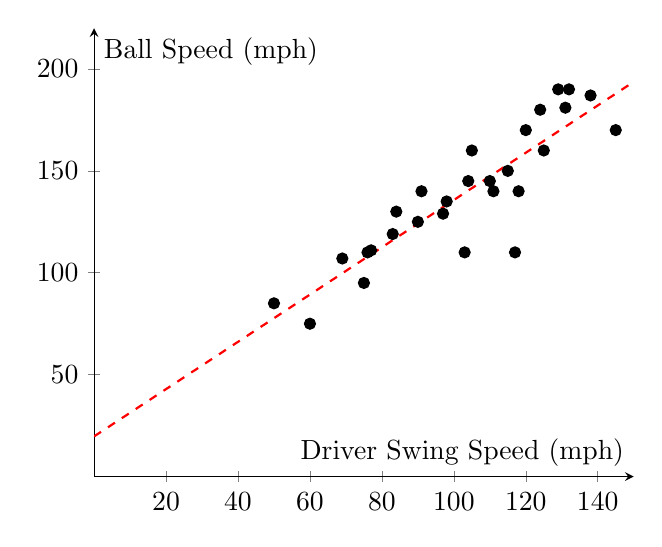
\begin{tikzpicture}
    \begin{axis}[
      xlabel=Driver Swing Speed (mph), 
      ylabel=Ball Speed (mph), 
      xmin=0, xmax=150,
      ymin=0, ymax=220, 
      legend style={at={(0.5,1.03)}, anchor=south, legend columns=2},
      axis lines=middle, 
    ]

    \addplot[only marks, mark=*] coordinates {
      (50, 85)
                (60, 75)
                (69, 107)
                (75, 95)
                (76, 110)
                (77, 111)
                (83, 119)
                (84, 130)
                (90, 125)
                (91, 140)
                (97, 129)
                (98, 135)
                (103, 110)
                (104, 145)
                (105, 160)
                (110, 145)
                (111, 140)
                (115, 150)
                (117, 110)
                (118, 140)
                (120, 170)
                (124, 180)
                (125, 160)
                (129, 190)
                (131, 181)
                (132, 190)
                (138, 187)
                (145, 170)
    };


    % Add the best-fit line (linear regression)
    \addplot[thick, color=red, domain=0:150, dashed] {1.16 * x +19.7};
    \end{axis}
  \end{tikzpicture}
  \caption{Scatter Plot of Data with Best-fit Line, Driver Swing Speed vs Ball Speed }
\end{figure}
This graph is a representation of the linear regression and most of the data points are scattered near the best-fit line except for a few points which are outliers. 
\begin{figure}[H] 
  \centering
  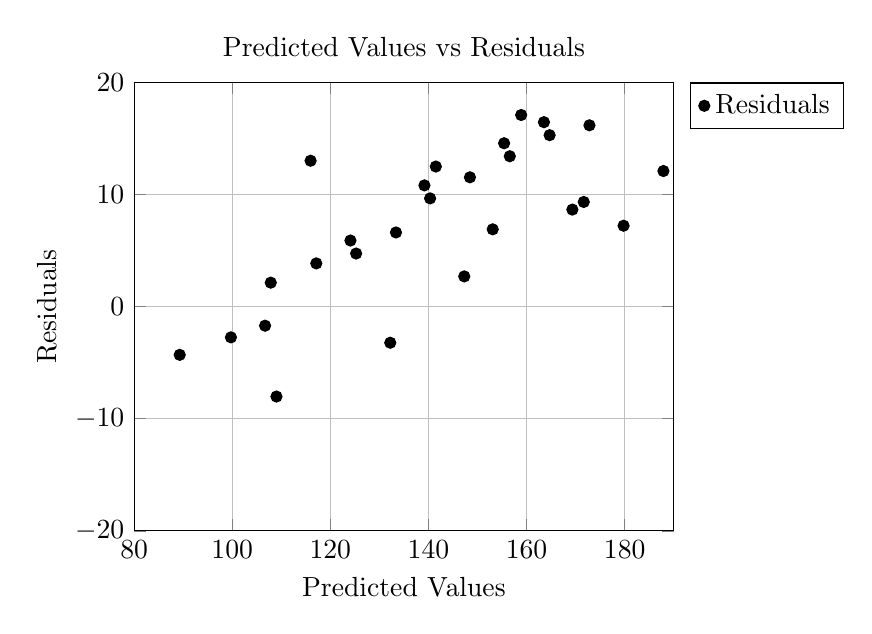
\begin{tikzpicture}
    \begin{axis}[
      xlabel={Predicted Values},
      ylabel={Residuals},
      title={Predicted Values vs Residuals},
      grid=major,
      legend entries={Residuals},
      legend pos=outer north east,
      xmin=80,  %
      xmax=190, % 
      ymin=-20, % 
      ymax=20   %
    ]
    
    % Predicted values
    \addplot[only marks, mark=*] coordinates {
      (89.3, -4.3)
      (99.74, -2.74)
      (106.7, -1.7)
      (107.86, 2.14)
      (109.02, -8.02)
      (115.98, 13.02)
      (117.14, 3.86)
      (124.1, 5.9)
      (125.26, 4.74)
      (132.22, -3.22)
      (133.38, 6.62)
      (139.18, 10.82)
      (140.34, 9.66)
      (141.5, 12.5)
      (147.3, 2.7)
      (148.46, 11.54)
      (153.1, 6.9)
      (155.42, 14.58)
      (156.58, 13.42)
      (158.9, 17.1)
      (163.54, 16.46)
      (164.7, 15.3)
      (169.34, 8.66)
      (171.66, 9.34)
      (172.82, 16.18)
      (179.78, 7.22)
      (187.9, 12.1)
    };
     \end{axis}
  \end{tikzpicture}
  \caption{Scatter plot of Predicted Values vs Residuals}
\end{figure}

\section{Conclusion}
\hspace{1em} To summarize, there is a high correlation between swing speed and ball speed, but as the swing speed goes up, there are some outliers in the data that can be caused by the position where the club hits the ball.
\section{Bibliography}
Matt. “Golf Club Distance Charts by Age, Gender and Skill Level.” Golf Sidekick, 12 Nov. 2023, www.golfsidekick.com/distance-finder/golf-club-distance-charts/. 

Staff, Swing Man Golf. “Average Golf Swing Speed Chart: Swing Man Golf.” Swing Man Golf | Just Another WordPress Site, 26 Feb. 2023, swingmangolf.com/average-golf-swing-speed-chart-2/. 

Sawant, Aamogh. “aamoghS/MathIA: MathIA Code.” GitHub, https://github.com/aamoghS/MathIA. . 
\end{document}
